\chapter{Lebenswirklichkeit von Afrodeutschen}\label{sec:3}
  \section{Afrodeutsch (Shirin Bediako)}\label{sec:3_1}
    \begin{flushleft}
    \end{flushleft}

    % \begin{center}
    %   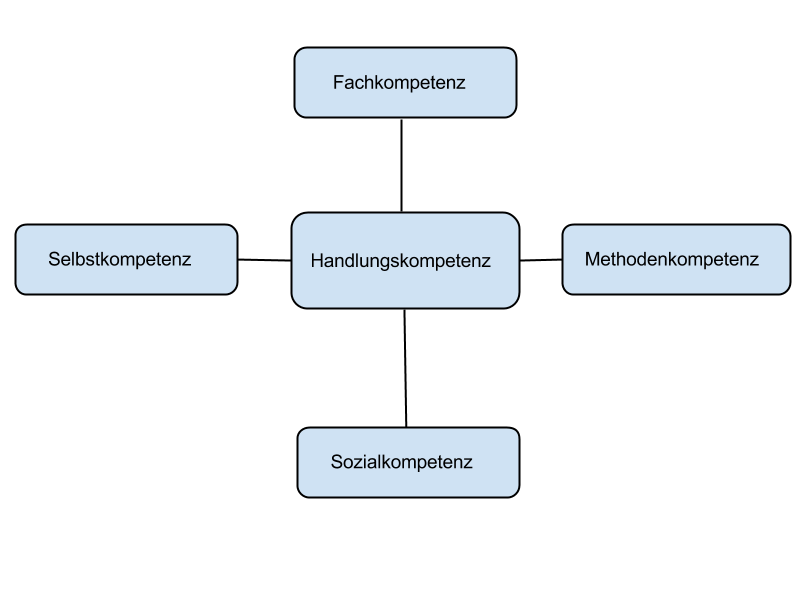
\includegraphics[width=0.85\textwidth]{grafik/taetigkeitspr.png}
    %   \captionof{figure}[Vierdimensionales Kompetenzmodell]{Vierdimensionales Kompetenzmodell \citep[vgl.][S.~15]{Kompet2011}}
    %   \label{fig:zusammenhang}
    % \end{center}

    \begin{flushleft}
    \end{flushleft}


  \section{Schwarzsein, Wei�sein - Deutschsein  (Shirin Bediako)}\label{sec:3_2}
    \begin{flushleft}
    \end{flushleft}

    \begin{flushleft}
    \end{flushleft}

    \begin{flushleft}
    \end{flushleft}


  \section{Mono- und Bikulturelle Familienstrukturen und Erziehungsstile (Shirin Bediako)}\label{sec:3_3}
    \begin{flushleft}
    \end{flushleft}

    \subsection{Deutsche Familien}\label{sec:3_3_1}
      \begin{flushleft}
      \end{flushleft}
      
    \subsection{Westafrikanische Familien}\label{sec:3_3_2}
      \begin{flushleft}
      \end{flushleft}
    
    \subsection{Westafrikanisch-deutsche Familien}\label{sec:3_3_3}
      \begin{flushleft}
      \end{flushleft}
      




    % \begin{flushleft}
    %   Eine Spielanalyse kann wie folgt aussehen:
    %   \begin{itemize}
    %     \item Inwieweit werden Kinder dazu ermutigt in diesem Spiel empathisch zu sein?
    %     \item Inwieweit werden verschiedene Rollen in diesem Spiel eingenommen und ausgehandelt?
    %     \item Wie sieht in diesem Spiel die Kontaktaufnahme unter den Kindern aus?
    %     \item Inwiefern ist es f�r dieses Spiel von N�ten, sich gegenseitig zu helfen und mit anderen zu kooperieren?
    %     \item Welche Regeln gibt es und m�ssen diese gegebenfalls mit den Kindern abgesprochen bzw. neu definiert werden?
    %   \end{itemize}
    % \end{flushleft}
